\section{CW 复形的同调}
\sourcepage{276--277}
现在说明怎样计算 CW 复形的奇异同调。本节始终以 $X$ 表示 CW 复形，开胞腔为 $e_\alpha$，特征映射为 $f_\alpha$。通常 $H_p$ 表示奇异同调；若 $X$ 可三角剖分，也可理解为单纯同调，因为两者之间有自然同构。

\entry{定义}{4.13.1}令 $D_p(X)=H_p(X^p,X^{p-1})$，并定义 $\partial:D_p(X)\to D_{p-1}(X)$ 为复合
\[
H_p(X^p,X^{p-1})\xrightarrow{\partial_*}H_{p-1}(X^{p-1})\xrightarrow{j_*}H_{p-1}(X^{p-1},X^{p-2}),
\]
其中 $j$ 为包含映射。因为 $H_{p-1}(X^{p-1})\xrightarrow{j_*}H_{p-1}(X^{p-1},X^{p-2})\xrightarrow{\partial_*}H_{p-2}(X^{p-2})$ 正合，所以 $\partial^2=0$。所得链复形 $\mathcal D(X)=\{D_p(X),\partial\}$ 称为 $X$ 的\textbf{胞腔链复形}。

\entry{例}{4.13.2}若 $X=|K|$，开胞腔取开单形，并用单纯同调计算，则 $C_i(K^{(p)},K^{(p-1)})$ 在 $i\ne p$ 时为零，在 $i=p$ 时等于 $C_p(K)$。因此 $H_p(X^p,X^{p-1})=C_p(K)$。胞腔边缘算子也正是单纯边缘算子。所以至少在这种情形，胞腔链复形确实计算 $X$ 的同调。

我们的目标是证明一般情形也类似：$D_p(X)$ 是以有向 $p$ 维胞腔为基的自由阿贝尔群，而且 $\mathcal D(X)$ 的同调同构于 $X$ 的奇异同调。先证明一系列引理。

\entry{引理}{4.13.3}任一 $p$ 维胞腔的特征映射 $f_\alpha:(B^p,S^{p-1})\to(\overline e_\alpha,\dot e_\alpha)$ 都诱导相对同调同构。

\sourcepage{278}
\textbf{证明：}零维时显然。设 $p>0$，记 $\widehat e_\alpha=f_\alpha(0)$。特征映射是商映射，其在饱和开集 $B^p\setminus\{0\}$ 上的限制仍为商映射。径向形变收缩将穿孔球收缩到 $S^{p-1}$，通过商映射 $f'_\alpha\times i_I$ 诱导 $\overline e_\alpha\setminus\{\widehat e_\alpha\}$ 到 $\dot e_\alpha$ 的形变收缩，见图 4.13.1。
\begin{center}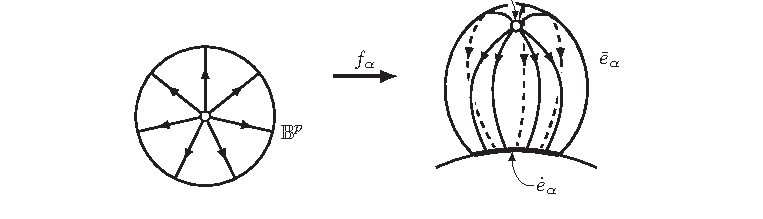
\includegraphics[width=.96\textwidth]{figures/4-13-1.pdf}\\图 4.13.1\end{center}
考虑下列交换图的两行空间偶，以及各列的特征映射：
\[
\begin{split}
(B^p,S^{p-1})\longrightarrow(B^p,B^p\setminus\{0\})
\longleftarrow(\Int B^p,\Int B^p\setminus\{0\}),\\
(\overline e_\alpha,\dot e_\alpha)\longrightarrow
(\overline e_\alpha,\overline e_\alpha\setminus\{\widehat e_\alpha\})
\longleftarrow(e_\alpha,e_\alpha\setminus\{\widehat e_\alpha\}).
\end{split}
\]
左侧两包含映射由形变收缩及定理 4.3.9 诱导同构；右侧两包含映射由切除分别删去 $S^{p-1}$ 和 $\dot e_\alpha$，也诱导同构。最右竖直映射是将 $0$ 映到 $\widehat e_\alpha$ 的同胚，所以最左竖直映射也诱导同构。\hfill$\square$

\entry{引理}{4.13.4}设 $f:X^{p-1}\amalg\coprod B_\alpha\to X^p$ 将骨架表示为由闭 $p$ 维球粘合而成的空间，$S_\alpha=\Bd B_\alpha$。则 $f$ 诱导
\[
H_i(\coprod B_\alpha,\coprod S_\alpha)\cong H_i(X^p,X^{p-1}).
\]

\sourcepage{279}
\textbf{证明：}与上一个引理类似。令 $0_\alpha$ 为各球中心，$\widehat e_\alpha=f(0_\alpha)$。商映射在删去所有球心后的饱和开集上的限制仍为商映射。该定义域可形变收缩到 $X^{p-1}\amalg\coprod S_\alpha$，并通过商映射诱导 $X^p\setminus\bigcup\{\widehat e_\alpha\}$ 到 $X^{p-1}$ 的形变收缩。考虑两行
\[
\begin{split}
(\coprod B_\alpha,\coprod S_\alpha)\to
(\coprod B_\alpha,\coprod(B_\alpha\setminus\{0_\alpha\}))\\
\longleftarrow(\coprod\Int B_\alpha,\coprod(\Int B_\alpha\setminus\{0_\alpha\})),\\[3pt]
(X^p,X^{p-1})\to(X^p,X^p\setminus\bigcup\{\widehat e_\alpha\})
\longleftarrow(\bigcup e_\alpha,\bigcup(e_\alpha\setminus\{\widehat e_\alpha\})).
\end{split}
\]
各列为 $f$。右列为一一对应的商映射，故为同胚；各横向包含映射由形变收缩或切除诱导同构，如上一证明，故得结论。\hfill$\square$

\entry{定理}{4.13.5}群 $H_i(X^p,X^{p-1})$ 在 $i\ne p$ 时为零，在 $i=p$ 时为自由阿贝尔群。若 $\gamma$ 生成 $H_p(B^p,S^{p-1})$，则各 $p$ 维胞腔的一组特征映射给出的 $(f_\alpha)_*\gamma$ 构成一组基。\translatornote{原书生成元所在群误印为 $H_p(B^p,S^p)$，球的边界应为 $S^{p-1}$。}

\textbf{证明：}由上一个引理，所求群同构于 $H_i(\coprod B_\alpha,\coprod S_\alpha)$。每个球在拓扑和中开且彼此不交，所以此群为 $\bigoplus_\alpha H_i(B_\alpha,S_\alpha)$。应用球的相对同调计算即得结论。\hfill$\square$

\entry{定义}{4.13.6}对三元组 $X\supset A\supset B$，短正合列
\[
0\to S_p(A)/S_p(B)\to S_p(X)/S_p(B)\to S_p(X)/S_p(A)\to0
\]
诱导\textbf{三元组的同调正合列}
\[
\cdots\to H_p(A,B)\to H_p(X,B)\to H_p(X,A)\to H_{p-1}(A,B)\to\cdots.
\]
其存在性是定理 3.3.8 的内容，也可由同调公理推出（第 3.5 节习题）。连续映射 $f:(X,A,B)\to(Y,C,D)$ 自然诱导两条正合列间的同态。

\sourcepage{280}
对 $(X,A,B)=(X^p,X^{p-1},X^{p-2})$，这个正合列中的连接同态恰为胞腔边缘算子。因为连接同态与包含映射 $j_*$ 可交换，它等于 $H_p(X^p,X^{p-1})\to H_{p-1}(X^{p-1})\to H_{p-1}(X^{p-1},X^{p-2})$。

为了以后使用，将证明一个稍一般的结果：空间写为递增子空间之并，以 $H_p(X_p,X_{p-1})$ 为链群、三元组的连接同态为边缘。在适当条件下，该链复形计算空间同调。

\entry{定义}{4.13.7}空间 $X$ 的\textbf{滤过}（filtration）是并为 $X$ 的递增子空间列 $X_0\subset X_1\subset\cdots$。空间连同滤过称为\textbf{滤过空间}。若连续映射 $f:X\to Y$ 满足 $f(X_p)\subset Y_p$，称其\textbf{保持滤过}。

\entry{定理}{4.13.8}设 $X$ 有上述滤过，$i<0$ 时令 $X_i=\varnothing$。假设 $H_i(X_p,X_{p-1})=0$（$i\ne p$），且每个紧子集包含于某个 $X_n$。令 $D_p(X)=H_p(X_p,X_{p-1})$，边缘由三元组连接同态定义，则有同构
\[
\lambda:H_p(\mathcal D(X))\to H_p(X),
\]
且对保持滤过的连续映射诱导的同态具有自然性。

\textbf{证明：}先看例 4.13.2 的单纯复形情形，$X_p$ 是 $p$ 维骨架，$\mathcal D(X)=\mathcal C(K)$。由于定义 $H_p(K)$ 只用到 $p+1,p,p-1$ 维链，亦有 $H_p(X)=H_p(K^{(p+1)},K^{(p-2)})$。下面先建立相应的一般结论。

\sourcepage{281}
\textbf{步骤 1。}证明包含映射诱导 $i_*:H_p(X_{p+1})\to H_p(X)$ 为同构。由正合列
\[
\begin{split}
H_{p+1}(X_{p+i+1},X_{p+i})\to H_p(X_{p+i})\to H_p(X_{p+i+1})\\
\to H_p(X_{p+i+1},X_{p+i}),
\end{split}
\]
在 $i\ge1$ 时两端为零，所以从 $X_{p+1}$ 开始，各后续骨架的 $p$ 维同调之间都是同构。

由紧支集性质，每个 $\beta\in H_p(X)$ 来自某个紧子集 $C$ 的同调，而 $C\subset X_{p+k}$，可取 $k\ge1$。于是 $\beta$ 来自 $H_p(X_{p+k})$，再由前述同构来自 $H_p(X_{p+1})$，证明满射。

若 $\beta\in H_p(X_{p+1})$ 在 $X$ 中变为零，则其代表链及使它成为边缘的有限奇异链具有紧载体，包含于某个 $X_{p+k}$。因此 $\beta$ 在 $H_p(X_{p+k})$ 中已为零；因前述映射为同构，$\beta=0$。这证明单射。

\textbf{步骤 2。}证明 $j_*:H_p(X_{p+1})\to H_p(X_{p+1},X_{p-2})$ 为同构。逐步加入相对子空间，考虑三元组正合列
\[
\begin{split}
H_p(X_i,X_{i-1})\to H_p(X_{p+1},X_{i-1})\to H_p(X_{p+1},X_i)\\
\to H_{p-1}(X_i,X_{i-1}).
\end{split}
\]
对 $i\le p-2$，两端均为零，故中间映射为同构。从空集依次加到 $X_{p-2}$ 即得结论。

\sourcepage{282}
\textbf{步骤 3。}对四元组 $X\supset A\supset B\supset C$，可把四个三元组正合列排成下图。取特殊情形 $(X,A,B,C)=(X_{p+1},X_p,X_{p-1},X_{p-2})$，则图中两个上角的群由假设为零。
\begin{center}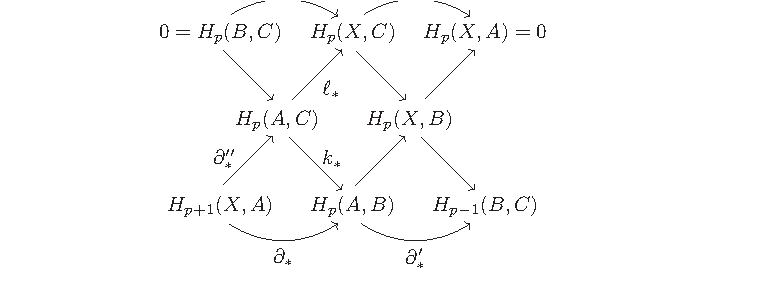
\includegraphics[width=.96\textwidth]{figures/4-13-diagram.pdf}\end{center}
映射 $k_*$ 将 $H_p(A,C)$ 同构地映到 $\ker\partial'_* $；$\ell_*$ 满射，所以 $\ell_*k_*^{-1}$ 将该核满射到 $H_p(X,C)$。由 $\ker\ell_*=\operatorname{im}\partial''_*$ 及图的交换性，其核恰为 $\operatorname{im}\partial_*$。因此
\[
\frac{\ker\partial'_*}{\operatorname{im}\partial_*}\cong H_p(X,C)=H_p(X_{p+1},X_{p-2}).
\]
更一般的图论证见第 3.5 节习题 1。结合前两步，
\[
H_p(X)\cong H_p(X_{p+1})\cong H_p(X_{p+1},X_{p-2})\cong H_p(\mathcal D(X)).
\]
若 $f$ 保持滤过，前两个同构显然与 $f_*$ 可交换，且 $f_*$ 将上述正合图映到 $Y$ 的相应图，故第三个同构也可交换。这证明自然性。\hfill$\square$

\sourcepage{283}
\entry{定理}{4.13.9}设滤过空间 $X=|K|$，每个 $X_p$ 为维数至多为 $p$ 的子复形的多面体，以单纯同调计算，并假定非对角相对同调均为零。则 $H_p(X_p,X_{p-1})$ 可视为 $C_p(K)$ 的子群，且上一定理的 $\lambda$ 由包含映射诱导。具体地，此子群是由 $X_p$ 承载、边缘由 $X_{p-1}$ 承载的所有 $p$ 维链。

\textbf{证明：}每个紧集在有限子复形中，而有限多个单形最终均包含于某个滤过阶段，故上一定理的紧集假设满足。$X_p$ 无 $(p+1)$ 维单形，所以相对 $p$ 维同调就是相对闭链群；$X_{p-1}$ 无 $p$ 维单形，所以 $C_p(X_{p-1})=0$。因此相对闭链恰是上述子群。

上一定理中，$\lambda$ 是将 $\ker\partial'_*$ 的元素沿 $k_*^{-1}$、$\ell_*$、$j_*^{-1}$、$i_*$ 依次映到 $H_p(X)$。这些同态均由包含映射诱导，故在此单纯链解释下，$\lambda$ 正是包含诱导的同态。\hfill$\square$

对每个 $p$ 维胞腔，群 $H_p(\overline e_\alpha,\dot e_\alpha)$ 为无限循环群，其两个生成元称为胞腔的两个\textbf{定向}。开胞腔连同一个定向称为\textbf{有向胞腔}。为每个 $p$ 维胞腔选择定向，再由包含映射送入 $H_p(X^p,X^{p-1})$，就得到胞腔链群的一组基。胞腔链复形的同调由上述定理同构于空间的奇异同调。

\sourcepage{284}
若 $X$ 可三角剖分，则每个胞腔闭包也是子复形的多面体。群 $H_p(\overline e_\alpha,\dot e_\alpha)$ 是由该闭包承载、边缘由 $\dot e_\alpha$ 承载的 $p$ 维单纯链群。它的任一个生成元称为这个空间偶的\textbf{基本闭链}（fundamental cycle）。胞腔链群的每个元素均可唯一写成有限个这样的基本闭链的整数线性组合。

\entry{例}{4.13.10}设 $X$ 是由矩形 $L$ 通常粘合得到的环面或 Klein 瓶。它有一个二维胞腔 $e_2$、两个一维胞腔 $e_1,e'_1$、一个零维胞腔。于是 $D_2\cong\Z$、$D_1\cong\Z\oplus\Z$、$D_0\cong\Z$。
\begin{center}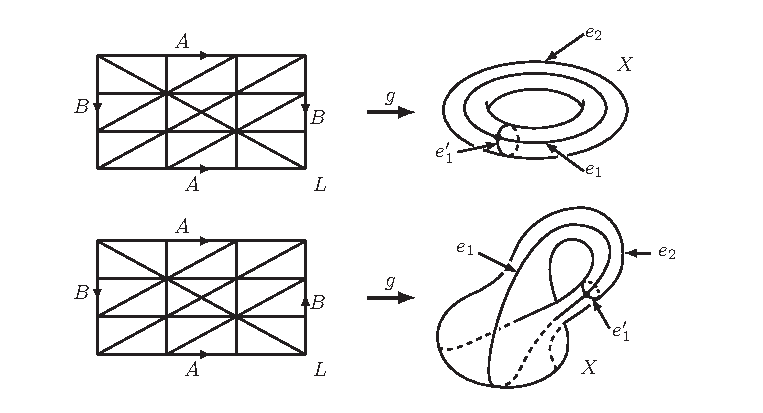
\includegraphics[width=.96\textwidth]{figures/4-13-2.pdf}\\图 4.13.2\end{center}
矩形中所有逆时针定向的二维单形之和 $d$ 是 $(L,\Bd L)$ 的相对闭链，且不是其他闭链的非平凡整数倍，所以为基本闭链。由引理 4.13.3，$\gamma=g_\#d$ 是二维胞腔的基本闭链。

\sourcepage{285}
令 $c_1,c_2,c_3,c_4$ 为图 4.13.3 中按箭头定向的边链。取 $w_1=g_\#c_1$、$z_1=g_\#c_2$ 为两个一维胞腔的基本闭链。计算
\[
\partial c_1=v_4-v_1,\qquad\partial c_2=v_2-v_1,\qquad
\partial d=-c_1+c_2+c_3-c_4.
\]
\begin{center}
\includegraphics[width=.96\textwidth]{figures/4-13-3.pdf}\\图 4.13.3\end{center}
两种空间均有 $\partial w_1=\partial z_1=0$。环面中，$g_\#c_1=g_\#c_3$、$g_\#c_2=g_\#c_4$，故 $\partial\gamma=0$。Klein 瓶中，第一等式不变，而 $g_\#c_2=-g_\#c_4$，故 $\partial\gamma=2z_1$。因此环面的同调为
\[
H_2\cong\Z,\qquad H_1\cong\Z\oplus\Z,\qquad H_0\cong\Z;
\]
Klein 瓶的同调为
\[
H_2=0,\qquad H_1\cong\Z\oplus\Z/2,\qquad H_0\cong\Z.
\]
这些计算以前做过；现在它们的依据是 CW 复形的一般定理，而不再是第 1.7 节中专门针对这些空间的论证。这正是胞腔理论使计算系统化的意义。

\sourcepage{286}
\entry{例}{4.13.11}设 $n>1$。球面有一个 $n$ 维胞腔及一个零维胞腔，故胞腔链群仅在这两维为无限循环群，其余为零。因此 $H_n(S^n)\cong\Z$、$H_0(S^n)\cong\Z$，其余为零。$n=1$ 时也可作类似计算。

\entry{定理}{4.13.12}设 $\mathcal C$ 是非负自由链复形，且 $H_0(\mathcal C)$ 自由、非零。则存在胞腔链复形同构于 $\mathcal C$ 的 CW 复形。习题 4 将引导证明此定理。

\subsection*{习题}
\begin{enumerate}
\item 将 $n$ 重环面连通和、$n$ 重实射影平面连通和表示为可三角剖分的 CW 复形，求胞腔链复形，重新计算其同调。
\item 设 $A\subset X$ 闭，且为 $X$ 中某个开集的形变收缩核。把 $A$ 压缩为一点所得空间记为 $X/A$，证明 $H_p(X,A)\cong\widetilde H_p(X/A)$。〔提示：考察引理 4.13.3 的证明。〕
\item 设 $A$ 为 CW 复形 $X$ 的子复形。证明包含映射诱导单射 $D_p(A)\to D_p(X)$，记商为 $D_p(X,A)$。
\begin{enumerate}[label=(\alph*)]
\item 若 $X$ 可三角剖分，证明 $\mathcal D(X,A)$ 计算相对单纯同调。〔提示：用长正合列证明包含到 $C_p(X,A)$ 的映射诱导同调同构。〕
\item 一般地，证明它计算相对奇异同调。〔提示：将它与链群为 $H_p(X^p\cup A,X^{p-1}\cup A)$、边缘来自三元组正合列的链复形认同。对所有整数 $p$ 令 $X_p=X^p\cup A$，重复定理 4.13.8 的证明，把绝对同调替换为相对于 $A$ 的同调。〕
\end{enumerate}
\item 按下列步骤证明定理 4.13.12。〔*〕
\begin{enumerate}[label=(\alph*)]
\item 若 $n\ge1$，证明对 $n$ 维单形 $\sigma$，任意同态 $H_n(\sigma,\Bd\sigma)\to H_n(S^n,x_0)$ 均由某个连续映射诱导。〔见第 3.4 节习题 3。〕
\item 若 $X$ 由一族只共用一点 $p$ 的 $n$ 维球面组成，$n>0$，证明任意 $\alpha\in H_n(X,p)$ 都是某个映射 $(S^n,x_0)\to(X,p)$ 所诱导的同态作用于生成元所得的像。
\item 对 $p>0$，证明可写 $C_p=U_p\oplus Z_p$，其中 $Z_p$ 为闭链群；零维可写 $C_0=\partial U_1\oplus A$，其中 $A\ne0$。
\item 完成证明。
\end{enumerate}
\item 设 $G_0,G_1,\ldots$ 是阿贝尔群列，$G_0$ 自由且非零。假设习题 4 的结论，证明存在 CW 复形 $X$，使所有 $H_i(X)\cong G_i$。
\end{enumerate}
